\section{Lei de Ohm e efeito Joule}

\frame{
	\frametitle{Lei de Ohm}
	\begin{block}{Inter-relação entre as variáveis de um circuito elétrico}
		Lembrando do exemplo do tanque...
		
		$$\text{Efeito} = \dfrac{\text{Causa}}{\text{Oposição}}$$
	\end{block}

	\medskip

	\centering
	
	\setmyunit{1cm}
	\begin{tikzpicture}
	\fill[blue] (0,0) -- ++(0,-3) -- ++(4,0) -- ++(0,0.5) -- ++(-1,0) -- ++(0,2.5) -- cycle;
	
	\draw (0,0) -- ++(0,-3) -- ++(4,0) ++(0,0.5) -- ++(-1,0) -- ++(0,2.5);
	
	\draw (0,0) -- +(0,0.5) (3,0) -- +(0,0.5);
	
	\draw[-Latex] (3,-2.75) ++(0,0.15) -- node[below=0pt] {Vazão} +(0.75,0);
	
	\draw[thick] (3.5,-2.5) -- ++(0,0.5) ++(0,0.4) circle (0.4);
	
	\foreach \x in {0,30,...,330}
	\draw (3.5,-1.6) ++(\x:0.35) -- +(\x:0.05);
	
	\draw (3.5,-1.6) -- +(25:0.4);
	
	\draw[decorate,decoration={brace,amplitude=10pt,mirror,raise=4pt}] (0,0) -- (0,-2.5) node[midway,left=15pt] {Altura};
	\end{tikzpicture}
	
%\centerline{\includegraphics[width=0.5\linewidth]{Figuras/Ch12/ohm2.png}}
}

\frame{
	\frametitle{Leis de Ohm}
	\begin{block}{1ª Lei de Ohm}
		Para um condutor mantido à temperatura constante, a razão entre a tensão entre dois pontos e a corrente elétrica é constante. Essa constante é denominada de resistência elétrica.
	\end{block}

	$$\boxed{I \triangleq \dfrac{U}{R}}$$
	
	\centering
	
	\setmyunit{2cm}
	\begin{circuitikz}
		\draw (0,0) to[battery,l=$ U $] ++(0,-1) -- ++(1,0) to[R,l=$ R $, *-*] ++(0,1) ++(-1,0) to[ammeter,i=$ i $] ++(1,0) (1,0) -- ++(0.5,0) to[voltmeter] ++(0,-1) -- ++(-0.5,0);
	\end{circuitikz}
	
%	\centerline{\includegraphics[width=0.5\linewidth]{Figuras/Ch13/1leiohm.PNG}}
}

\frame{
	\frametitle{Leis de Ohm}
	\begin{block}{2ª Lei de Ohm}
		A resistência de um fio é diretamente proporcional ao seu comprimento e inversamente proporcional à sua área de secção transversal. A constante de proporcionalidade que estabelece a igualdade para a equação da Segunda Lei de Ohm é a resistividade do material ($\rho$).
	\end{block}
	$$\boxed{R = \rho \dfrac{L}{A}}$$
	
	\setmyunit{1cm}
	
	\bigskip
	
	\centering
	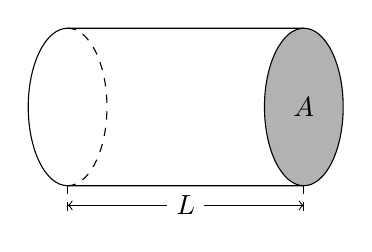
\begin{tikzpicture}
		\filldraw[black!30!white,draw=black] (3,-1) circle (0.5 and 1);
		
		\draw (0,0) -- (3,0) ++(0,-2) -- ++(-3,0) arc (-90:-270:0.5 and 1);
		
		\draw[dashed] (0,0) arc (90:-90:0.5 and 1);
		
		\node[] at (3,-1) {$ A $};
		
		\draw[dashed] (0,-2) -- +(0,-0.4) (3,-2) -- +(0,-0.4);
		\draw[<->] (0,-2.25) -- node[fill=white] {$ L $} +(3,0);
	\end{tikzpicture}
%	\centerline{\includegraphics[width=0.4\linewidth]{Figuras/Ch13/2leiohm.PNG}}
}

\frame{
	\frametitle{Potência Elétrica}
	\begin{block}{Corrente e tensão sozinhas não suficientes}
		\begin{itemize}
			\item Lâmpada $60$W x $100$W
			\item Pagamento de conta de luz às concessionárias
		\end{itemize}
	\end{block}

	\begin{block}{Definição}
		\textbf{Potência} é a quantidade de trabalho realizado em um determinado período de tempo.
	\end{block}
	$$P \triangleq \dfrac{\tau}{\Delta t}$$
	\begin{block}{Por que?}
		$$\boxed{P = U \cdot I}$$
	\end{block}
}

\frame{
	\frametitle{Exemplo prático}
	\centerline{\includegraphics[width=0.6\linewidth]{Figuras/Ch13/enel.png}}
}

\frame{
	\frametitle{Efeito Joule}
	\begin{block}{Definição}
		Ao existir corrente elétrica as partículas que estão em movimento acabam colidindo com as outras partes do condutor que se encontra em repouso, causando uma excitação que por sua vez irá gerar um efeito de aquecimento. A este efeito dá-se o nome efeito Joule.
	\end{block}

	\begin{block}{Efeito Joule e o efeito na potência}
		Como o resistor dissipa a energia em forma de calor, a potência total do sistema diminuiu.
	\end{block}
}

\frame{
	\frametitle{Efeito Joule}
	\centerline{\includegraphics[width=0.5\linewidth]{Figuras/Ch13/joule.jpg}}
	\begin{block}{Exemplo}
		A lâmpada de filamento incandescente funciona graças ao efeito Joule - o filamento aquece com a passagem da corrente elétrica e libera energia em forma de luz e calor.
	\end{block}
}

\frame{
	\frametitle{Efeito Joule}
	\centerline{\includegraphics[width=0.7\linewidth]{Figuras/Ch13/ferro.jpg}}
}

\frame{
	\frametitle{Efeito Joule}
	\begin{block}{Fórmula matemática}
		A potência elétrica dissipada em um resistor ôhmico é diretamente proporcional ao quadrado da intensidade da corrente \\
		$$\boxed{P = R \cdot I^2}$$
	\end{block}
}

\section*{Exercícios}

\frame{
	\frametitle{Exercícios}
	\begin{block}{}
		01. Em uma torradeira elétrica, vem marcados os valores de \SI{1000}{\watt} e \SI{27}{\volt}. Determine: \\
		(a) a intensidade de corrente que atravessa a torradeira. \\
		(b) o consumo de energia elétrica do aparelho, admitindo que ele permaneça ligado durante 2 horas.

		\vspace{0,5cm}

		02. Um aquecedor de água é submetido à d.d.p. $U = \SI{40}{\volt}$, sendo então percorrido por uma corrente elétrica $I = \SI{0.2}{\ampere}$. Determine: \\
		(a) a potência elétrica que se dissipa no aquecedor. \\
		(b) a energia elétrica dissipada após 3 minutos. \\
		(c) a resistência elétrica do resistor do equipamento.

		\vspace{0,5cm}

		03. Calcule a resistividade de um condutor que submetido a uma d.d.p. de \SI{100}{\volt}, passa uma corrente de \SI{10}{\ampere}. Seu comprimento é de \SI{10}{\meter} e a área da seção reta é de \SI{0.5}{\milli\meter\squared}.

	\end{block}
}

\section*{Referências}

\frame{
	\frametitle{Referências e Exercícios Complementares}
	\begin{itemize}
		\item Física, Ciência e Tecnologia – Vol 3. PENTEADO, Paulo César M; TORRES, Carlos Magno A. Ed. Moderna (2006)
	\end{itemize}
	%\centering{\alert{Página 36 - \textbf{1.6.1 até 1.6.5, 1.6.17 até 1.6.19}}} \\
	\centering{\alert{Lista de exercícios 13}}
}